\documentclass{report}
\usepackage{gensymb}
\usepackage{caption}
\usepackage{subcaption}
\usepackage{breqn}
\usepackage{pgfplotstable}
\usepackage{array}
\usepackage{booktabs}
\usepackage{graphicx}
\usepackage{url}
\usepackage{siunitx}
\usepackage{hyperref}
\hypersetup{
    colorlinks,
    citecolor=black,
    filecolor=black,
    linkcolor=black,
    urlcolor=black
}
\graphicspath{ {images/} }
\begin{document}
\title{
	{Detailed Analysis of the Relationship between Geometry and Airflow in Older Chinese Adult Male Nasal Cavities}\\
	{\large SAMME}\\
	{\includegraphics{rmit.jpg}}
}
\author{Sean Read}
\date{Day Month Year}
\begin{titlepage}
    \begin{center}
        \vspace*{1cm}
        
        \Huge
	\textbf{Detailed Analysis of the Relationship between Geometry and Airflow in older Chinese Adult Male Nasal Cavities}
        
        \vspace{1.5cm}
        
        \textbf{Sean Read}
        
        \vfill
        
        \vspace{0.8cm}
        
        \includegraphics[width=0.4\textwidth]{rmit}
        
        \Large
        SAMME\\
        RMIT\\
        Australia\\
        Date
        
    \end{center}
\end{titlepage}

\chapter*{Abstract}
Abstract goes here

\chapter*{Dedication}
To Mum and Dad, Chris, Coka, Gary, Paper \& Leigh

\chapter*{Declaration}
I declare that..

\chapter*{Acknowledgements}
I want to thank my supervisors, Dr Kiao Inthavong and Professor Jiyuan Tu and my cat

\tableofcontents

\newpage
\listoffigures
\listoftables

\chapter{Introduction}

\section{Background}

The ageing global population behooves a greater interest and investment in research and innovation in the area of geriatrics. One area of particular significance within the field of geriatrics is that of geriatric rhinology. A range of dysfunctions and aberrations from the normal functioning of healthy adults have been observed in the nasal cavities of elderly populations\cite{Edelstein1996, Lindemann2008}. These aberrations are liable to impact significantly on the quality of life of the sufferers. The nasal cavities of elderly citizens have been shown by previous researchers to show increased volume\cite{Kalmovich2005}. Alterations in histiological function have also been shown\cite{HO2001}. The extent to which functional aberrations are caused by geometric variations remains unclear\cite{Varga-Huettner2013}. The occurrence of respiratory diseases in the elderly is markedly higher than that found in younger populations\cite{HO2001, Edelstein1996}. It has been suggested that these higher recorded rates could be due in part to the impaired air conditioning functionality\cite{Lindemann2008}.

particle toxicology is an area which has been receiving increasing interest in recent decades. The potential health issues related to the inhalation of environmental hazards are multifarious and often life threatening. In order to minimise the physical cost to society of both man made and natural environmental toxins an understanding of the mechanisms by which the contaminants are being introduced in to the human body is imperative.

The use of computational fluid dynamics (CFD) to analyse nasal cavity flow dynamics is an area which has been receiving significant research attention in recent years. CFD simulations allow the achievement of highly detailed results with information covering a range of areas for a given fluid system at a minimal cost. Some of the more significant areas The use of 3d medical imaging techniques such as computed tomography (CT) scans in collaboration with CFD has facilitated the use CFD modeling techniques to approximate numerically fluid mechanism parameters of anatomically accurate models taken from models produced in vivo. This allows for more detailed comparisons of the effects of topological variations on the relevant fluid mechanisms.


The analysis of highly accurate models facilitated by the use of ct scans presents an opportunity for the analysis of inter-demographic variations in nasal cavity functionality. To date numerous inter-demographic studies have been carried out using CFD analysis of 3d models reconstructed from ct scan data. These demographic studies have included several focusing on age, however these age related studies have all focused on the variations between children and adults.


\section{Research questions and objectives}

In light of the information posed above, the following questions seem pertinent:

\begin{itemize}

  \item How do changes in nasal cavity geometry - caused by age - influence its airflow mechanisms?

  \item How do the same changes impact on heat and vapour transfer within the cavity?

\end{itemize}

To answer the aforementioned questions, the following objectives have been outlined:

\begin{itemize}

  \item reconstruct a series of nasal cavity geometries from medical scans that represent a spread of geometric characteristics [such as volume and surface area] across the norm. The existing literature shows a clearly defined relationship between age and volume: these models will serve as a representation of the aging population to be analysed compuationally.

  \item Model airflow across the series of reconstructed nasal cavities using computational fluid dynamic using a steady state assumption; defining inlet conditions to approximate a resting rate of respiration. 

  \item Compare the simulation results between geometries. A variety of post processing methods have been employed to compare various aspects of fluid mechanic functionaility of the nasal cavity models. The literature has shown clear discrepencies in the functionality of nasal cavities as a function of age; it is our intention through these measurements to examine in more detail the extent of these variations.

  \item  Compare results with existing results from various experimental methods from the previously extant literature. The results of the post processing Will be used to explain discrepancies in nasal functionality observed by previous researchers.

\end{itemize}
 
\section{Research outline}

Developments medical image reconstruction technologies now allow researchers to reconstruct highly detailed, digital 3d representations of various anatomical structures from ct scans. When coupled with CFD simulations, this presents an unprecedented capacity for in depth analysis of physiological fluid flow mechanisms.

This study aims to use CFD analysis of CT scan data from the nasal cavities of a range of Asian males to investigate the impact of the age induced expansion of the nasal cavity on the air-conditioning functionality of the nasal cavity. Air flow mechanisms, heat transfer rates and humidification efficacy is analysed. The Data is then discussed - in the context of the rhinological symptoms attributed by previous researches to elderly patients - in order to arrive at a more precise understanding of the role of nasal geometry in the presentation of said symptoms.

This study represents, to the best of our knowledge, the first in depth, mechanistic, computational study undertaken into the role of nasal geometry in common rhinological symptoms associated with the aging process.


\chapter{Literature review}


\section{Geriatric rhinology}
The common rhinological complaints of the elderly include dryness, runny noses, crusting and epistaxis\cite{Varga-Huettner2013}. Epidemiological studies have been carried out to examine the consistency of the manifestation of various symptoms throughout elderly patients with mixed results. The literature at present seems to be unanimous on the tendency of the nasal cavity's cross sectional area to increase with age. Several researchers have investigated this phenomena using acoustic rhinometry and shown good concordance in study outcomes\cite{Kalmovich2005, Edelstein1996,WhanKim2007,Lindemann2008}. Nasal air heating and humidification have been examined vivo and shown to be impacted by age\cite{Lindemann2008}. Increases in postnasal drip, nasal drainage, sneezing, coughing, olfactory dysfunction and gustatory rhinitis with age were observed in a clinical study of 131 patients\cite{Edelstein1996}. The results on the impact of aging on the quality of life have not been unanimous, a 2009 study found that in a sample of 80 people no significant relationship could be observed between age and nasal discomfort\cite{Lindemann2010}. The same study, however, concurred with previous results on the increase of volume and cross sectional area as a function of age. Changes with in the nose appear to not be limited to the increased volume. Both functional and structural variations in the respiratory epithelium have been observed with age, contributing to slower clearing of the mucous\cite{HO2001}. Functional variations in air conditioning capabilities have been shown in vivo\cite{Lindemann2008}, with statistically significant reductions in relative humidity and heat transfer observed in elder nasal cavities. The level to which this is attributable to change in histological function as opposed to variations in the fluid mechanisms as a result of the expansion of the cavity remains to be investigated.

\section{Experimental}
The anatomy of the nasal cavity was first classified in detail by Emil Zuckerlandl in the 19th century\cite{Stammberger1989}. Anatomically, his records were more or less up to the standard of what can be assessed from modern scanning techniques\cite{Stammberger1989}, however the investigation of airflow characteristics was still severely limited by technological capacity\cite{Eccles2000}. It was not until the turn of the 19th century that experimentation in to nasal airflow began in proper\cite{Eccles2000}. The experimental methods used to examine airflow in the human nasal cavities in the last century have been numerous. Some of the more common in vivo techniques used include rhinomanometry, which allows measurement of the pressure drop across the nasal cavity\cite{Hilberg1989} and acoustic rhinometry, which allows measurement of the cross sectional area of the nasal cavity as a function of depth\cite{Hilberg1989}. Ultimately, however, direct detailed measurements of flow mechanics within the human nasal cavity taken in vivo are not viable with current technology as a result of the complexity and small scale of the nasal geometry\cite{Doorly2008c}. Thus the preferred media for the testing in modern times has tended to be either physical or computational models reconstructed from ct scan data\cite{Doorly2008c}. The physical models that have been constructed from ct scan data are able to provide high detail on fluid flow properties when compared with older techniques such as rhinomanometry\cite{Ma2009}, however such experimental set ups are costly to run in terms of time and resources, in particular when compared with the high level of detail that can be achieved from a well done CFD simulation\cite{Ma2009}.

\subsubsection{Image reconstruction}
the use of ct scans to reconstruct accurate 3D models of various aspects of the human physiology cite ??? (look at references from Dongs' book, ask Kiao about the relevance of this chapter)

\section{Computational Fluid Dynamics}
Computational fluid dynamics(CFDs) is a discipline which is principally concerned with the computational approximation of solutions to the navier stokes equations for closed fluid systems\cite{Tu2008}. In many fields - inlcuding rhinology - CFD has facilitated economical and detailed investigations in to cases in which experimental investigation would otherwise be costly or, in cases such as rhinology, impossible\cite{Keyhani1995}.

CFDs were the primary driving force behind the development of larger and faster computers until the 80's\cite{Wendt2009}. In more, recent times, the continuing advancement of computational technologies has facilitated considerable growth in the scope and accuracy of CFDs for predicting the behaviour of increasingly complicated systems\cite{Tu2008}. 

One of the areas of investigation that has been facilitated by these advances is that of nasal airflow. Initially, simplified nasal cavity geometry models used to create computational meshes and solve numerically for the fluid flow properties under steady state conditions\cite{Keyhani1995, Hahn1993}. Later 3d models extracted from CT scans were used to achieve more accurate results\cite{Martonen2002}. In addition to this, various inlet and outlet conditions have been compared, chiefly the difference between and unsteady  which model the variations in flow as a function of time throughout the nasal cycle\cite{Shi2006} or an assumed constant velocity, time independent, steady state assumption based model\cite{Wen2008}. This discrepancy has been a point of much contention, and it seems that the current position is that this decision depends on the application at hand\cite{Doorly2008c}. Certainly to date it seems that the vast bulk of the case studies comparing different geometries have used the steady state assumption\cite{Xi2012, Zhu2011, Garcia2007}

Another issue which has been of some debate in the literature is the relevance of the inclusion of sinuses in the modelled flow domain. It has been reasonably commonplace to include the sinuses in studies that are examining the effects of sinus surgery\cite{Xiong2008a, Lindemann2005}. Also it has been shown that, while the impact on airflow is relatively minimal, the sinuses can be subject to not insignificant levels of particle deposition for particles in the range of 1 nanometre in diameter, and particularly for low flow rates\cite{Ge2012}. The added  requirements in time and computational complexity necessitated by the inclusion of the sinuses, however, seems to warrant their exclusion from models in situations where they are not specifically relevant\cite{Doorly2008c}



\section{Airflow structures}
Airflow structures have been investigated and portrayed through a variety of both qualitative and quantitative methods. The earliest papers prior to the widespread use of cfd's focused primarily on the pressure drop over the nostrils as measured with rhinomanometry\cite{Martin1981}. Modern technological innovation has facilitated the development of a range of techniques for both visualisation of airflows and the quantification of their various characteristics. In particular the range of data that can be obtained from numerical simulations is vast and detailed, and so the question of how to interpret it becomes particularly important.

One more commonly used visualisation method is the use of streamlines cite fig streamlines, often coloured by velocity\cite{Wen2008, Zhu2011, Garcia2007}. These are useful for showing flow distribution as well as significant recirculation zones\cite{Lintermann2013, Xi2014}. Another commonly used method, shown in figure ref fig velocity contours is coronal cross sectional contours portraying velocity These contours may or not include streamlines to help highlight the presence of vortices in the flow\cite{Wen2008}. Another method, presented in \cite{Lintermann2013} uses a $\Delta $ criterion to trace the vortices present in the flow structure. In \cite{Lintermann2013}, these are then coloured by variables related to turbulence and vorticity in order to provide a deeper insight in to the vortex structure behaviour.

Quantitative methods for analysing and comparing air flow structures seem to be less standardised. Prior to the invention of modern imaging and investigative techniques, rhinologists relied on readings of cross sectional area and pressure from techniques such as rhinomanometry and acoustic rhinometry\cite{Doorly2008c}. The detailed flow information that can be extracted from ct scan models either experimentally or computationally opens up a much wider range of options in terms of quantitative analysis. Pressure is still often included as it is said to provide an insight in to the inspirational efficiency of the cavities\cite{Lintermann2013}. Pressure is often plotted as a function of flow rate in order to provide a point for validation by comparison with experimental set ups\cite{Wen2008, Inthavong2014}. In addition, it is can be analysed as a function of longitudinal position in order to gain an insight in to the relationship between the geometric variations and pressure drop\cite{Lintermann2013}. Another common technique is velocity distribution measurement\cite{Keyhani1995, Zhu2011, Lintermann2013}. This can include a cross sectional zone by zone analysis\cite{Keyhani1995, Zhu2011}, which has been suggested to be useful for the measurement of the efficacy of olfaction\cite{Zhu2011}, or by longitudinal sections\cite{Lintermann2013,Taylor2010} . Another commonly used quantitative measure is wall shear stress. Wall shear stress is also analysed in a variety of different ways. Distributions are analysed longitudinally\cite{Wen2008} and around the cross sectional parameter of the relevant chapter of the nasal cavity\cite{Burgos2014}. These measurements have been shown to be significant for predicting heat and mass transfer within the regions\cite{Taylor2010}, and thus their longitudinal and parametric distributions are significant understanding the distribution of such mechanisms.

\section{Demographic studies}
To date the variation of nasal cavity functionality has been compared between several demographics have been investigated in the literature. The previously investigated demographics include  age\cite{Xi2012}, which can then be subclassified into children\cite{Xi2012} and the elderly\cite{Lindemann2008}. Both of these have been investigated through both in vitro\cite{Weinhold2004} and in vivo\cite{Kalmovich2005, Edelstein1996, WhanKim2007, Lindemann2008} techniques. Child models have also been investigated computationally\cite{Xi2012}. The variations that have been observed in children's nasal airway functionality has been suggested to be linked to particle filtration ability \cite{Xi2012}. It seems plausible that this effect could be significant also in the case of elderly models. Cross sectional areas have been graphed as a function of radial position to compare the geometries of different models in many studies\cite{Xi2012, Zhu2011, Lindemann2008, Garcia2007}. Surface area has also been suggested to be significant metric in predicting flow behaviour, as surface area to volume ratios are expected to impact on the flow behaviour\cite{Xi2012, Garcia2007} resistance across the nasal cavity, measured as pressure drop, is also often used as a predictor of flow behaviour within the nasal cavity\cite{Edelstein1996, Lindemann2008, WhanKim2007}. Streamlines are a commonly used method for visualising flow structures in nasal cavity models\cite{Xi2012, Garcia2007, Zhu2011}. Sectional flow flux has also been used to 
***analysis of comparison techniques***


\section{Heat and vapour transfer}

Earlier investigations in to the heat and vapour transport characteristics of the nasal cavity used a straight pipe model as a simplification of the nasal cavity geometry\cite{Ingelstedt1961}. The first experiments involving real nasal cavity geometries were carried out in the 80s, using cast models taken from cadavers\cite{Nuckols1983}.

In vivo experiments into temperature variation across the nasal cavity have been done using various temperature measuring devices; modern experiments have tended towards using thermocouples because they are small and respond quickly\cite{Elad2008}. For measuring humidity in vitro, modern researchers have tended towards the use of capacitative temperature sensors\cite{Keck2000}. Detailed profiles of temperature and humidity throughout the nasal cavity have been presented by several past researchers\cite{Keck2000}.

CFD's have been used to simulate heat and vapour transfer in the nasal cavities with good accordance with experimental results\cite{Lindemann2004}. Early simulations investigating heat and vapour transfer used a steady state assumption for inflow conditions\cite{Naftali1998}. Later, the effect of the nasal cycle on temparature distributions were investigated, showing significant variations in the nasal temperature distributions throughout the nasal cycle\cite{Elad2006}.

Cross sectional temperature contours have been used to visualise the distribution of temperature throughout the nasal cavity; this provides a clear way of visualising the distribution\cite{Naftali2005}. Saggital heat flux contours have also been used to similar effect\cite{Sullivan2013}. Heat flux, temperature, water flux and humidity have all been mapped as a function of saggital position in the nasal cavity\cite{Garcia2007, Sullivan2013, Yu2014}. The nasal valve has been noted from these observations to be a region of particular significance to heat and vapour transfer mechanisms\cite{Sulivan2013}. 




%\cite{Elad2008}
%
%in vitro studies - blood and mucous as transport agents for heat and moisture. Ingelstedt and Tolmalm, 1961, straight pipe simulation. Casting plastic Nuckols et al 1983, napthalene sublimation - Hanna and scherer, 1986. 
%
%In vivo studies - limited due to complexity of geometry, posterior Temperature 31-34 deg C, 90-95\%, Keck et al 2000 a, b. Variation of the nasal mucosa temperature, turbulence linked to higher heat flux values - Lindemann et al 2002. Temporal change in cavity flow - Eccles 2000; Hanif et al. 2000
%
%Computational - accurate 3d replica for predicting temperature distribution - Lindemann et al 2004, 2006, Pless et al 2004a, 
%
%Naftali et al. 2005, full 3d model for heat and vapour transfer in anatomical replica
%
%Wolf et al 2004 - psychometric charts used to calculate required heat and water to condition incoming air
%
%Naftali et al 2005 - varied inlet conditions show similar conditining capacity
%
%Kastl et al - impact of rhino-surgical interventions
%
%Influence of septal deviations - Pless et al. 2004b
%
%
%\cite{Garcia2007}
%
%Heat flux adjusted for evaporation as per (40)
%
%100\% RH at wall due to mucus
%
%vestibule zero water flux
%
%ambient air at 50\% RH, outflow at outlet
%
%mapped temperature across cavities, also relative humidity, water flux contours
%heat flux and water flux against length. Also as a function of height from nasal floor
%
%Tables of water flux per unit area
%
%flow partitioning
%
%pressure drop


\section{Literature gap}

To date, to the best of our knowledge, although some research has been carried out on the effects of aging on nasal airflow, CFDs have not been used to examine in depth the influence of age related variations in nasal cavity geometry on flow structure or heat and vapour transfer characteristics. 

%\section{Particle filtration}
%
%



\chapter{Model Reconstruction and Meshing} \label{MRM}

\section{Introduction}

The first step towards the computational analysis of older nasal cavities is the obtainment of computer models to describe their geometry. In this section the reconstruction process by which such computer models were obtained for the purpose of this thesis is explained.

\section{Geometry}
\subsection{Introduction}

The reconstruction of nasal cavity model computer models- including discretisation - can be divided into 5 stages: image aquisition, data conversion, segmentation, refinement and meshing. Firstly medical imaging technologies are used to extract a series of pixelated slices, in which the various materials which make up the human body can be identified by variation in greyscale measurements. These slices are then interpolated to create a 3D structure of voxels (the 3D equivalent of a pixel).

The reconstruction of the nasal cavity geometries can be very time consuming and prone to human error. The improvement on and automation of the reconstruction process are areas of active research. This chapter presents an overview of the methods in current use for the various phases (mentioned above) by which a nasal cavity geometry is prepared for computational solution.

\subsection{Non-invasive medical imaging}

There are various forms of medical imaging that can be used for the identification of the nasal cavity geometry. Here we briefly overview Computed Tomography (CT), the form of medical imaging used for the nasal cavity geometries presented in this thesis.

CT scans use a series of x-rays taken at regular intervals within the region of interest. x-ray scans use photons sent in beams through the region of interest; these photons interact differently with the material that they encounter depending on its density. Electronic detectors feed the photon pattern emitted from the body in question to a computer, which uses this information to create images. These images are made up of pixels which are each assigned a grey scale value based on their x-ray attenuation coefficient. In medical imaging the Hounsfield scale is used, whereas in image processing the greyscale is numbered from black to white between 0 to 255. Figure \ref{fig:greyscale} shows an  example of how greyscale values are assigned to pixels in a CT image.

\begin{figure} 
  \includegraphics[width=1\textwidth]{grayscale.png}
\caption{example of how greyscale values are assigned to pixels in a CT image} \label{fig:greyscale}
\centering
\end{figure}
 
\subsection{Image segmentation} 

Once the CT scan has been outputted as a series of voxels, the anatomical geometries relevant to the project at hand need to be extracted. To achieve this goal, the voxels that make up the relevant section of the data need to be identified somehow. This can be done manually - by going through the many slices that make up the CT scan and identifying the relevant areas - however this process is extremely time consuming.

Numerous algorithms have been developed for the purpose of automating the process of image segmentation; all of which have certain advantages and disadvantages. For the most part these algorithms can be subsumed in to three categories, presented below (in order of increasing complexity):

\begin{description}

  \item[\textbf{Thresholding}] regions are identified and separated according their  greyscale value. This is the simplest algorithm for defining regions.
 
  \item[\textbf{Edge detection}] either local maxima of the first derivite of intensity or zero values of the second derivative are used to identify region edges. Edge detection tends to reduce the noise when compared with thresholding
 
  \item[\textbf{Region based}] regions are grown from the inside out. This produces more coherent regions, but is unable to detect regions that are segregated.

\end{description}

These methods and many more exist and are in active development; many of them are available for free online. The implementation of such algorithms from first principles, however is quite a complex procedure. Fortunately many of these algorithms have already been implemented in software packages - of which commercial and open source variations are available - which are specifically compiled for working with medical imaging outputs. 
 
\subsection{Preparation of model for meshing}

Once the region in question has been extracted from the medical imaging output, it can be saved as some CAD format. There are certain criteria that need to be fulfilled by a CAD model before it can be read by 3D meshing software and used to create a mesh. It is often the case when the data is exported from the medical imaging software that it is 'dirty'; that there are contradictory or arbitrary elements in the geometry. These elements need to be removed through the use of CAD software before the geometry is suitable for the creation of a useable 'clean' 3D mesh. Note that the geometry needs to contain also topological information in order to create a watertight mesh. The details of the process by which the geometry is prepared for meshing are described in Figure \ref{fig:segchart}.


\begin{figure}
  \includegraphics[width=1\textwidth]{flowchart.png}
\caption{Flow chart showing the process by which an anatomical geometry is prepared - with the help of medical imaging software - for solution via CFD codes} \label{fig:segchart}
\centering
\end{figure}
 
\subsection{Summary} 

Anatomical geometry reconstruction - including that of the nasal cavity - begins with medical imaging of the area in question. The geometry is then extracted from the medical imaging data using one (or several) of the available extraction algorithms outlined above. After extraction, cleaning of the geometry with CAD software is generally necessary to ensure that the geometry is water-tight and 'clean' before it can be meshed. This chapter has given an overview of some of the more pertinent methods in current use for the reconstruction of anatomical geometries from medical imaging data. Figure \ref{fig:cavzamp} shows an example of the construction process. 

Figure \ref{fig:geo} shows the models reconstructed for and used in this thesis. They have been labeled NC for nasal cavity plus a number. The first cavity, NC04, is 48 years old and was reconstructed by a colleague earlier and used in this thesis as a comparison point for the older models. The other models are aged between 60 and 78. All of the models are of healthy Asian males. In this case we chose only healthy Asian males as to minimise the impact of demographic variations other than age on the presented geometries.

\begin{figure} 
  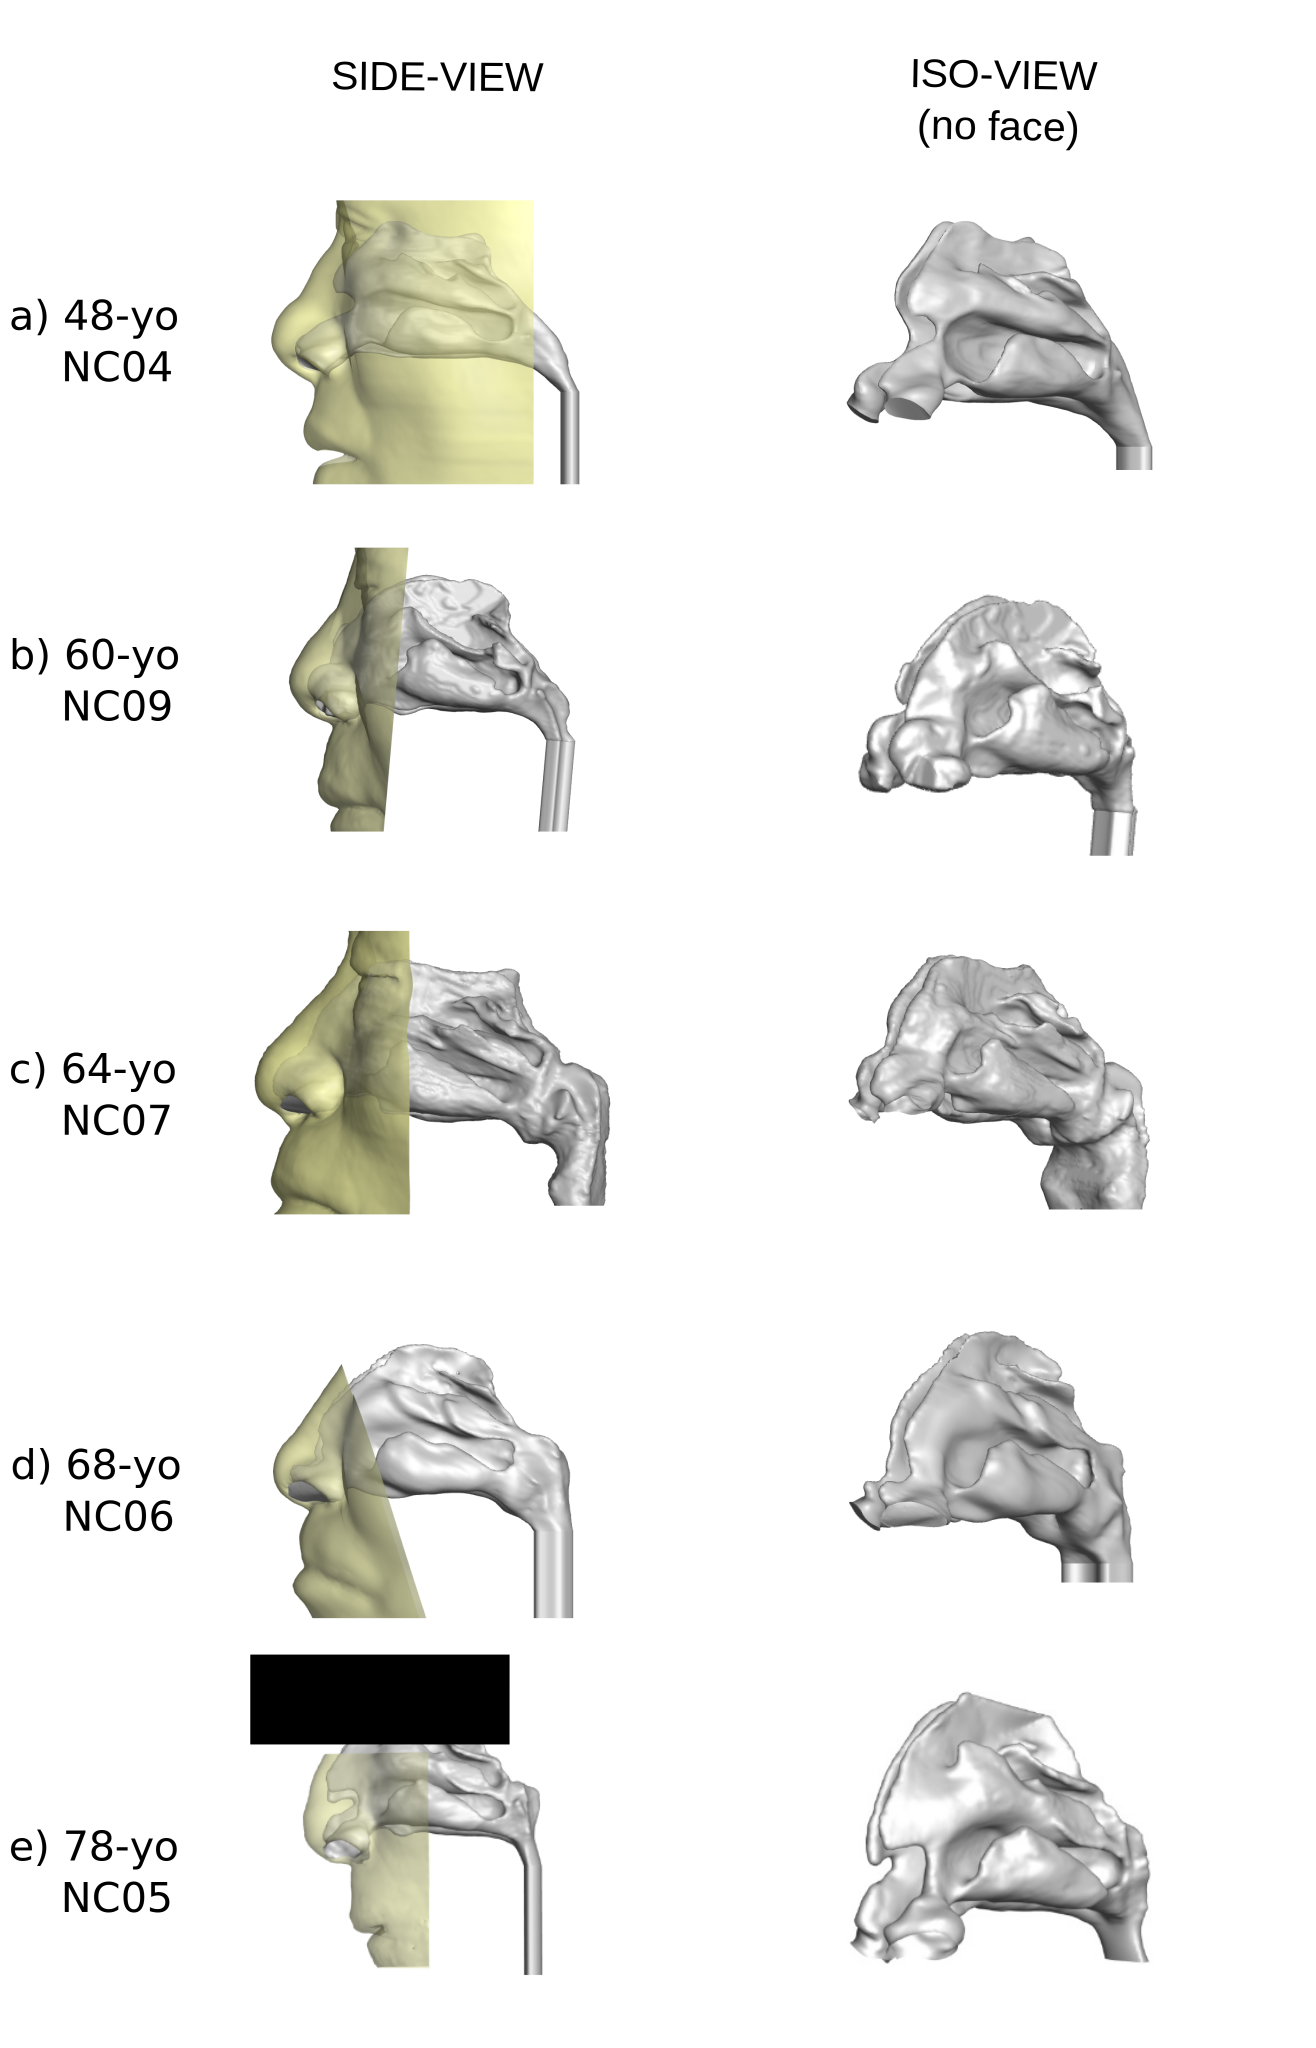
\includegraphics[width=0.8\textwidth]{geometries}
  \caption{geometries of the five cavities used for analysis in this thesis}
  \label{fig:geo}

\end{figure}
\begin{figure}[t!]

  \begin{subfigure}[t]{0.5\textwidth} 
    \includegraphics[width=\textwidth]{slicer}
    \caption{}
    \label{fig:slicer}
  \end{subfigure}%
  ~ %
  \begin{subfigure}[t]{0.5\textwidth} 
    \includegraphics[width=\textwidth]{geomagic}
    \caption{}
    \label{fig:geomag}
  \end{subfigure}

  \caption{example of nasal cavity geometry generation: \ref{fig:slicer} shows an example of the extraction of a 3D model from CT scan data, using, in this case, an open source software package, slicer. Figure \ref{fig:geomag} shows the refined geometry extracted from the CT slices seen in figure \ref{fig:cavzamp} (\subref{fig:slicer})}
  \label{fig:cavzamp}
\end{figure}
 
\section{Meshing} \label{Meshing}
\subsection{Introduction}

The navier stokes equations, upon which CFD is based (see chapter \ref{cfd}), is unsolvable (in most instances), except by approximation. In order to approximate a solution to a given system, its geometry must be approximated, or discretised, as a series of points. The process by which these points are defined and related to one another is known as meshing; this in itself is a complex discipline under active research. In this chapter current methods are reviewed, and guidelines are given for developing quality meshes.
\subsection{Mesh types} \label{mtypes}

There are many types of mesh that can be employed; all of them have their own advantages and disadvantages. 

\begin{description}
  \item[\textbf{Structured meshes}]
    are divided into segments of uniform size and shape. They are characterised by cells posessing either four nodal corner points in two dimensions, or eight in three dimensions. The points are mutually orthogonal and cartesionally defined. Being defined in this relatively simple way facilitates a higher level of computational efficiency. They are, however, limited in the level of structural complexity that they can accomodate.

  \item[\textbf{Unstructured meshes}] 
    The geometries encountered in the respiratory system are generally too complex to be effectively discretised in a structured manner; in cases such as these unstructured meshes can be used to acommodate the complexities of the given geometry. Unstructured meshes - usually constructed from triangles or tetrahedra - do not fit a regular pattern, and they do not have coordinate lines corresponding to curvilinear directions. Because of this, the solving of computations over unstructured domains is generally more computationally intensive; however with modern advances in computers this has become less significant an issue in many cases.

  \item[\textbf{Hybrid meshes}] 
    One disadvantage to the use of unstructured meshes is that they tent to show less accuracy near the wall. One commonly applied solution is the use of hexahedral elements near the wall, with the rest of the volume filled with unstructured - usually tetrahedral - elements. This method tends to improve the accuracy of near wall computations. One draw back of this method is that the prism layers can break down in the vicinity of excessively contoured walls. In this study this is the mesh type that is employed.

\end{description}

\begin{figure}
  \begin{subfigure}[t]{0.3\textwidth}
    \includegraphics[width=\textwidth]{ogrid}
      \caption{structured o-grid}
    \label{strucmesh}
  \end{subfigure}%
  ~%
  \begin{subfigure}[t]{0.3\textwidth}
    \includegraphics[width=\textwidth]{unstructuredmesh}
    \caption{unstructured}
    \label{unstrucmesh}
  \end{subfigure}%
  ~%
  \begin{subfigure}[t]{0.3\textwidth}
    \includegraphics[width=\textwidth]{hybridmesh}
    \caption{hybrid}
    \label{unstrucmesh}
  \end{subfigure}

  \caption{examples of the mesh types described in section \ref{mtypes}} 
  \label{fig:struct}
\end{figure}

\subsection{Meshing algorithms}
There are various meshing algorithms available, each with its own strengths and weaknesses. For the purpose of this study, an octree algorithm was selected. Octree algorithms work by repeatedly dividing The volume in to smaller sections, until the given criteria, for example mesh size, is fulfilled. This method is generally considered to be a relatively simple but robust approach to mesh generation. One drawback, however is that it can cause irregular element distributions near the boundary.

\subsection{Quality}

The quality of a generated mesh is dependant on its warp angle, skewness and aspect ratio. For a quadrilateral cell, as shown in figure \ref{fig:mqual}, the aspect ratio of the cell is defined as $AR = \frac{\Delta y} {\Delta x}$. Within the interior region, the $AR$ should be maintained within the range $0.2 < AR < 5$. This can be somewhat relaxed, however, in the vicinity of the wall.

Mesh skewness is defined as the extent to which it deviates in shape from the ideal. This is a square for quadrilateral cells, or an equilateral triangle for triangle or tetrahedral cells. It is defined for triangles and tetrahedrals as $\frac{\theta ideal - \theta actual} {\theta ideal}$ (see figure \ref{fig:mqual} for theta).

Many grid generation packages contain specific algorithms and/or functions for improving mesh quality. The gradient of mesh size variation should not exceed 1.2, as higher variations can cause problems in convergance.

\begin{figure}
  \includegraphics[width=1\textwidth]{mqual}
  \caption{Example of mesh cell with spacing $\Delta x$ , $\Delta y$ and angle $ \theta $ between the grid lines along with high $AR$ triangular and quadrilateral elements } \label{fig:mqual}
\end{figure}
 
\subsection{Mesh independence}

A significant source of error in the solution of CFD problems is derived from the discretisation process; when a system is separated into a number of finite elements, for the purpose of Numerical solution, the solution that is obtained from its solution is an approximation. It is necessary, then, to ascertain the required resolution, or mesh size, required to calculate a result that approximates the exact solution to a satisfactory degree of accuracy. This is done by means of a mesh independence test. This entails the monitoring of one - or several - fluid flow parameters of interest to the study over a series of mesh resolutions for the relevant system. Independence is said to have been achieved when the effect of mesh size on the selected flow variable(s) has become sufficiently insignificant. Figure \ref{fig:mind} shows the results from the mesh independence test conducted for smallest and the largest of the five models presented in this thesis.

\begin{figure}

  \begin{subfigure}[t]{0.5\textwidth}
    \includegraphics[width=\textwidth]{NC05mi}
    \caption{NC05 (78yo)}
    \label{fig:mi5}
  \end{subfigure}%
  ~%
  \begin{subfigure}[t]{0.5\textwidth}
    \includegraphics[width=\textwidth]{NC07mi}
    \caption{NC07 (64yo)}
    \label{fig:mi7}
  \end{subfigure}
  \caption{mesh independence test carried out for the largest and smallest of the new models presented in this thesis} \label{fig:mind}

\end{figure} 

\subsection{Meshing of the nasal cavity} 

Here we provide an overview of the meshing process applied to one of the nasal cavity models presented in this thesis. The process was the same for the other four models.

The system is divided in to three parts. The first of these surrounds the facial geometry directly adjacent to the nostrils; this is to allow for the developement of a more realistic inlet profile. The second is the nasal cavity itself. The third section is an pipe-like extension from the exit of the nasopharynx; this allows for the developement of a more realistic outlet profile, in a similar manner to the section around the inlet. This system can be seen in Figure \ref{fig:cavme} (\subref{fig:mesh1}).

The three stages of mesh refinement can be seen in Figure \ref{fig:cavme} (\subref{fig:mesh2}); The mesh resolution is much coarser in the external domain, refined closer to the inlet and then is most fine in the cavity itself, the area of interest. Note the use of hybrid mesh, with internal tetrahedral elements and close to wall prism layers, shown clearly in Figure \ref{fig:cavme} (\subref{fig:mesh4}).

\begin{figure}
  \begin{subfigure}[t]{0.5\textwidth}
    \includegraphics[width=\textwidth]{mesh2}
    \caption{whole system with face, extension from outlet and external zone}
    \label{fig:mesh1}
  \end{subfigure}%
  ~%
  \begin{subfigure}[t]{0.5\textwidth}
    \includegraphics[width=\textwidth]{mesh1}
    \caption{intersection of three mesh resolutions}
    \label{fig:mesh2}
  \end{subfigure}

  \begin{subfigure}[t]{0.5\textwidth}
    \includegraphics[width=\textwidth]{mesh3}
    \caption{cross section of cavity mesh}
    \label{fig:mesh3}
  \end{subfigure}%
  ~%
  \begin{subfigure}[t]{0.5\textwidth}
    \includegraphics[width=\textwidth]{mesh4}
    \caption{prism layer of cavity mesh}
    \label{fig:mesh4}
  \end{subfigure}
  \caption{mesh of NC06 (68yo)} \label{fig:cavme}
\end{figure}


  \begin{table} 
    \centering
  \pgfplotstableset{
  every head row/.style={before row=\toprule,after row=\midrule},
  every last row/.style={after row=\bottomrule}}

  \pgfplotstabletypeset[
      fixed zerofill,
      precision=2,
      display columns/0/.style={string type},
      display columns/1/.style={string type},
      display columns/1/.style={column name={Mesh size ($\times 1e06$)}},
      display columns/2/.style={string type},
      display columns/3/.style={string type},
      display columns/4/.style={string type},
      col sep=comma]{tables/Mesh.txt}
  \caption{parameters of the meshes for the nasal cavity models presented in this thesis}
  \label{tab:pvv}
\end{table}


\chapter{CFD fundamentals} \label{cfd}

\section{Fluid dynamics}
The aim of Computational fluid dynamics is to approximate numerically the physical conservation laws of newtonian physics:

\begin{itemize}
  \item conservation of mass

  \item The conservation of momentum (Newton’s second law, the rate of change of momentum equals the sum of forces acting on the fluid);

  \item The conservation of energy (first law of thermodynamics, the rate of change of energy equals the sum of rate of heat addition to and the rate of work done on the fluid).

\end{itemize}

    \subsection{Mass Conservation}

    The principle of conservation of mass is that, in a closed system, the mass remains constant. This means that fluid will move through a set region in such a way the mass is conserved. For an incompressible flow, this means that the outflows and the inflows will be equal. This can be written as
    \begin{equation} \label{eq:1}
      0 = \sum_{in} \dot{m} - \sum_{out} \dot{m}
    \end{equation} 

    Where $\dot{m}$ = mass flow rate.
    
    The mass flow rate can be written as $ \rho u A $,  for $\rho$ = density, $u$ = velocity and A is the scross sectional area of the flow. For flow in the x direction, $ A = \Delta z \Delta x $. For a two dimensional flow, $ \Delta z = 1 $, giving:

    \begin{equation} \label{eq:2}
      \dot{m}_{in} = \rho u \Delta y
    \end{equation}

    Extending this to equation \ref{eq:1}, in the x direction, for an incompressible flow we get

    \begin{equation} \label{eq:3}
      0 = \rho u_{in} \Delta y_{in} - \rho u_{out} \Delta y_{out}
    \end{equation}

    This can easily be extrapolated to three dimensions.
\begin{figure}   
  \centering
  \includegraphics[width=0.5\textwidth]{CompDom}
  \caption{Fluid moving through the computational domain, the inflow of ambient air must be equal to the air entering the lungs}
  \label{fig:CompDom}
\end{figure}
    In the case of the nasal cavity, this can be conceptualised in relation to the nasal cavity geometry, where the air flow rate going in to the nostrils must be equal to that leaving through the extension from the nasopharynx, as seen in figure \ref{fig:CompDom}.



    \subsection{Momentum Conservation}

    Momentum conservation is based on the Newton's second law:

    \centerline{$\sum F = ma$}

    Here $m$ is the mass of the system, $a$ is its rate of acceleration, and  $\sum F$ is the sum of forces acting on the system. F can generally be divided in to body and surface forces. Rewriting the mass as the product of volume and the density, and acceleration as the first derivative of velocity:


    \begin{equation} \label{eq:4}
      \sum F_{body} + \sum F_{surface} = (\rho \Delta x \Delta y \Delta Z) \frac{DU}{Dt}
    \end{equation}

    Body forces generally include gravity, centrifugal, Coriolis and electromagnetic forces; these all act on the volume from a distance.

    Surface forces are those that act directly on the surface of a fluid element. These fluid forces include normal stress, in the x direction $\sigma_{xx}$, which is made up of pressure forces $p$ exerted on the body and normal viscous stress components $tau_{xx}$; and tangential stresses, $\tau_{xy}$ and $\tau_{xz}$.

    Summing these forces in the x direction, for a 2D fluid element we get:
    

    \begin{dmath} \label{eq:5}
      \sum F_{surface, x} = [\sigma_{xx} \Delta y \Delta z - (\frac{\delta \sigma_{xx}}{\delta x} \Delta x) \Delta y \Delta z] 
      + [(\tau_{xy} + \frac{\delta \tau_{yx}}{\delta y} \Delta y) \Delta x \Delta z - \tau_{yx} \Delta x \Delta z]  
      = - \frac{\delta \sigma_{xx}}{\delta x} \Delta x \Delta y \Delta z + \frac{\delta \tau_{yx}}{\delta y} \Delta x \Delta y \Delta z
    \end{dmath}


    Assuming that the fluid is Newtonian and isotropic, $\sigma_{xx}$ can be related to pressure $p$ and viscous stresses $\tau_{xx}$ by

    \centerline{$\sigma_{xx} = -p + \tau_{xx}$}

    For a Newtonian fluid, stress-strain relations can be described as 

    \begin{equation} \label{eq:6}
      \tau_{xx} = 2 \mu \frac{\delta u}{\delta x} \quad \tau_{yx} = \mu \frac{\delta u}{\delta y}
    \end{equation}

    Where $\mu$ is the viscocity of the fluid. Combining equations \ref{eq:4} , \ref{eq:5} and \ref{eq:6} in the x direction, and cancelling out the volume term:

    \begin{equation} \label{eq:7}
      \rho \frac{Du}{Dt} = - \frac{\delta p}{\delta x} + \mu (\frac{\delta^2 u}{\delta x^2} + \frac{\delta^2 u}{\delta y^2}) + \rho \sum F_{b}
    \end{equation}
    
    Here the acceleration term is the total derivative of u, defined as the combined local and advection inertial forces, which in two dimensions can be written as

    \begin{equation} \label{eq:8}
      \frac{Du}{Dt} = \frac{\delta u}{\delta t} + v \frac{\delta u}{\delta y} + u \frac{\delta u}{\delta x}
    \end{equation}

    combining equations \ref{eq:7} and \ref{eq:8} and dividing through by $\rho$:

    \begin{equation} \label{eq:9}
      \underbrace{\frac{\delta u}{\delta t}}_{local\ acceleration} + v \underbrace{\frac{\delta u}{\delta y} + u \frac{\delta u}{\delta x}}_{convection} = - \underbrace{\frac{1}{\rho} \frac{\delta p}{\delta x}}_{pressure gradient} + \underbrace{\nu (\frac{\delta^2 u}{\delta x^2} + \frac{\delta^2 u}{\delta y^2})}_{diffusion} + \underbrace{\sum F_{b}}_{body force}
    \end{equation}

    Where $\nu$ is kinematic viscocity, defined as $\frac{\mu}{\rho}$. 

    \subsection{Energy Conservation}

    Conservation of energy is derived from the first law of thermodynamics, that in a steady flow system the total energy of a control volume remains constant; that inflows and outflows must be equal. This can be expressed analogously to the mass conservation as 

    \begin{equation} \label{eq:10}
      \frac{DE}{Dt} = \sum{\dot{Q}} + \sum{\dot{W}}
    \end{equation}

    Where $\dot{Q}$ is heat transfer and $\dot{W}$ is the rate of work done. $E$ is energy per unit mass and is expressed as

    \centerline{$E = C_{p} T$}

    $\frac{DE}{Dt}$ can be expressed similarly to Equation \ref{eq:8}:

    \begin{equation} \label{eq:11}
      \frac{DE}{Dt} = \frac{\delta E}{\delta t} + v \frac{\delta E}{\delta y} + u \frac{\delta E}{\delta x} = C_{p} (\frac{\delta T}{\delta t} + v \frac{\delta T}{\delta y} + u \frac{\delta T}{\delta x})
    \end{equation}

    For a 2D element, the total energy can therefore be calculated from

    \begin{equation} \label{eq:12}
      \rho \frac{DE}{Dt} \Delta x \Delta y = \rho   C_{p} (\frac{\delta T}{\delta t} + v \frac{\delta T}{\delta y} + u \frac{\delta T}{\delta x}) \Delta x \Delta y
    \end{equation}

    From Fourier's law of heat conduction, for a 2D system we can write

    \begin{equation} \label{eq:13}
      \dot{Q}_{x} = k A_{x} \frac{\delta T}{\delta x} = \dot{q}_{x} A_{x} = \dot{q}_{x} \Delta y
    \end{equation}

    where $\dot{q}$ is heat flux = $\dot{Q}/A$

    The heat transferred into the element can thus be expressed as

    \begin{equation} \label{eq:14}
      [q_{x} + \frac{\delta q_{x}}{\delta x}] \Delta y - q_{x} \Delta y = \frac{\delta q_{x}}{\delta x} = k \frac{\delta^2 T}{\delta x^2} \Delta x \Delta y
    \end{equation}

    \begin{figure} \label{fig:eneq}
      \caption{Flow of heat energy through a 2D element}
    \end{figure}

    reconstructing equation \ref{eq:10} with the inclusion of \ref{eq:14}, considered also in the y direction, we can cancel out the volume term:

    \begin{equation} \label{eq:15}
      \underbrace{\frac{\delta T}{\delta t}}_{local\ acceleration} + \underbrace{u \frac{\delta T}{\delta x} + v \frac{\delta T}{\delta y}}_{convection} = \underbrace{\frac{k}{\rho C_{p}} ( \frac{\delta^2 T}{\delta x^2} + \frac{\delta^2 T}{\delta y^2} )}_{diffusion}
    \end{equation}

\section{Humidity}

One of the primary functions of the nasal cavity is the humidification of the incoming air in preparation for its interaction with the lungs. It therefore stands that any investigation into the fluid mechanisms of the nasal cavity would be incomplete without adressing the efficacy of this function. One simple but effective method for approximating humidification data in a computational domain is the use of the convection-diffusion equation.

Analogously to equations \ref{eq:15} and \ref{eq:9}, for a 2D element we can write

\begin{equation} \label{eq:16}
  \underbrace{\frac{\delta C_{H_{2} O}}{\delta t}}_{local acceleration} + \underbrace{u \frac{\delta C_{H_{2} O}}{\delta x} + v \frac{\delta C_{H_{2} O}}{\delta y}}_{convection} = \underbrace{D_{H_{2} O} ( \frac{\delta^2 C_{H_{2} O}}{\delta x^2} + \frac{\delta^2 C_{H_{2} O}}{\delta y^2} )}_{diffusion}
\end{equation} \nocite{Naftali1998}

Where $C_{H_{2} O}$ is the concentration of water vapour and $D_{H_{2} O}$ is the diffusivity of water in air.

\begin{figure} \label{fig:h2oel}
  \caption{water vapour moving through a 2D element}
\end{figure}

\section{Solving the governing equations}

The conservation equations outlined earlier in this chapter are nonlinear partial differential equations which, for complex domains such as the nasal cavity geometry, have no analytical solution; they must therefore be approximated algebraically and solved numerically.

\subsection{Discretisation}

Approximating, or discretising a system to make it numerically solvable can be done in many ways. One of the more common methods in modern solvers is the finite volume method, which can be applied to unstructured as well as structured meshes, making it particularly suited to complex geometries such as that of the nasal cavity.

The Finite Volume Method discretises the system into a series of volumes. The fluxes of relevant variables through the different faces of each element are then treated as a discrete system, which is able to be solved numerically.

\begin{figure}
  \includegraphics[width=\textwidth]{unstrfv}
  \caption{representation of mesh discretised with finite volume method}
  \label{usfv}
\end{figure}

Finite volume methods can tend to cause artificial, or numerical, diffusion if the mesh is of low quality. It is thus necessary to follow proper meshing practices, similar to those outlined in section \ref{Meshing}.

\subsection{Numerical Solution}

Once the system has been discretised, a system of linear equations can be developed to describe the system. These equations can be solved with one of several methods. These methods can generally be divided into two categories: either direct or iterative. In general, for large complex domains such as the nasal cavity models presented in this paper, iterative methods are the only way to derive a solution.


\chapter{Results}

\section{Introduction}
A large amount of information can be obtained from the results of a thorough CFD simulation. The challenge then becomes to present it in a way that is clear and comprehensible.
This chapter presents the analysis of the simulation results for the fluid systems defined by the nasal cavity models reconstructed for the thesis.

\section{Geometry Variations}


\begin{figure}
\centering
\includegraphics[width=0.7\textwidth]{regions}
\caption{Colour coded display of the regional divisions used in tables \ref{tab:secvol}, \ref{tab:secsa}, \ref{tab:deff}} 
\label{fig:regions}
\end{figure} 

One-hundred cross-sectional slices were taken from the nostrils tip to the nasopharynx. From nostrils tip to choanae, vertical slices were made, while angled slices were made in the nasopharynx until the slice became horizontal (Figure \ref{fig:Slices}).


\begin{figure} 
\centering
\includegraphics[width=0.7\textwidth]{slicesSchematic}
\caption{Representation of the slicing method used for sampling data across the sagittal axis throughout this thesis} 
\label{fig:Slices}
\end{figure}

Figure \ref{fig:sil} shows 8 coronal slices taken at equidistant spacing across the sagittal axis between the anterior vestibule and the nasopharynx. We see the airway elongate vertically which increases the perimeter length while maintaining a relatively constant surface area. This area to perimeter ratio has been cited as an important factor in the development of fluid flow in the nasal cavity. The thinner cavities also tend to exhibit higher wall shear stress. This is because of the steeper velocity gradients, which create stress through the viscosity of air, near the wall. This narrowness is also likely to influence heat and vapour transfer in the cavities; when the cavities are narrower there is less distance for the heat and vapour to travel from the wall to saturate the incoming air, and so it is likely to saturate the airflow more comprehensively. The variation in cavity thickness between the cavities can also be clearly observed in this figure.


\begin{figure} 
  \includegraphics[width=\textwidth]{Silhouettes}
  \caption{Cross sectional silhouettes taken at evenly spaced intervals across the sagittal axis of  the cavities between the vestibule and nasopharynx}
  \label{fig:sil}

\end{figure}

Figure \ref{fig:area} shows the cross sectional area as a function of normalised distance along the sagittal axis. The distance has been normalised between the entrance to the nostrils and the end of the nasopharynx. A sample of cavities from the pre-existing literature has also been included for comparison. A significant variation can be seen in the average cross sectional area of the models presented in this paper; This variation is most pronounced towards the rear of the cavities. None of the models show quite the same volume as the atrophic rhinitis model, also shown here as Garcia \cite{Garcia2007}, prior to the nasopharynx, although the 64yo is close. The general shape of the curve is reasonably similar for the various models in this paper, with notable exceptions in the Nasopharynx of the 64yo cavity and a larger spike in the vestibule region of the 78yo. Observations from Figure 3 can be compared with the cross sectional silhouettes from Figure 2, for a clearer understanding of the variations in geometry between the 4 models presented here. The range of cross-sectional areas allows us to observe the relationship between various fluid mechanical properties of the cavity and cavity volume/cross-sectional area.


\begin{figure}
  \includegraphics[width=\textwidth]{Areavsdistance}
  \caption{Area versus distance across the four nasal cavities with a series of examples from the literature}
  \label{fig:area}
\end{figure}



Table \ref{tab:secvol} - \ref{tab:deff} shows the variation of the volume, surface area and effective diameter respectively, in comparison with models from the literature. The volumes of the four models presented in this paper varied significantly. The largest discrepancies were noted in the pharynx and turbinate regions, with a less marked discrepancy in the vestibular region. The 48 – yo is showing greater volume than that seen in the atrophic rhinitis patient from \cite{Garcia2007}. The surface area of the atrophic rhinitis model is also significantly lower, to the extent that the effective diameter, shown in Table \ref{tab:deff}, is larger than the models presented in this paper.

\begin{table}
  \begin{tabular}{p{0.125\textwidth}p{0.1\textwidth}p{0.1\textwidth}p{0.1\textwidth}p{0.1\textwidth}p{0.1\textwidth}p{0.11\textwidth}p{0.13\textwidth}}
 & \textbf{48yo, NC04} & \textbf{78yo, NC05} & \textbf{68yo, NC06} & \textbf{64yo, NC07} & \textbf{60yo, NC09} &\textbf{Xi et al. \cite{Xi2012}} & \textbf{Garcia et al.\cite{Garcia2007}} \\
\cline{2-8}
\textbf{Turbinal region} & 18.54 & 22.78 & 24.62 & 30.722 & 16.73 & 12.63 & 33.66\\
\textbf{Naso-pharynx}  & 3.84 & 5.40 & 12.80 & 20.09 & 4.57 & 16.33 & 10.60\\
\textbf{Vestibule} & 3.10 & 4.15 & 2.81 & 4.21 & 7.39 & 5.50 & 2.41\\
\textbf{Total} & 25.48 & 32.33 & 40.23 & 55.07 & 28.69 & 34.43 & 47.77 \\
\hline
\end{tabular}
\caption{ Sectional volume, according to sections as seen in Figure \ref{fig:regions} ($\mathrm{cm^3}$)}\label{tab:secvol}
\end{table}
\begin{table}
  \begin{tabular}{p{0.125\textwidth}p{0.1\textwidth}p{0.1\textwidth}p{0.1\textwidth}p{0.1\textwidth}p{0.1\textwidth}p{0.11\textwidth}p{0.13\textwidth}}
 & \textbf{48yo, NC04} & \textbf{78yo, NC05} & \textbf{68yo, NC06} & \textbf{64yo, NC07} &\textbf{60yo, NC09}& \textbf{Xi et al.} & \textbf{Garcia et al.}\\
 \cline{2-8}
\textbf{Turbinal region} & 170.92 & 174.07& 190.44 & 163.44 & 138.80 & 112.59 & 133.50\footnote{includes vestibule} \\
\textbf{Naso-pharynx} & 12.20 & 12.80 & 25.23 & 40.42 & 11.37 & 40.93 & 31.46\\
\textbf{vestibule} & 15.71 & 17.37 & 12.45 & 17.92 & 46.96 & 35.58 &  -\\
\textbf{total} & 198.82 & 204.25 & 228.11 & 221.79 & 197.192 & 189.10 & 164.96\\
\hline
\end{tabular}
\caption{Sectional surface area, according to sections shown in Figure \ref{fig:regions}($\mathrm{cm^2}$)}\label{tab:secsa}
\end{table}
\begin{table}
  \begin{tabular}{p{0.125\textwidth}p{0.1\textwidth}p{0.1\textwidth}p{0.1\textwidth}p{0.1\textwidth}p{0.1\textwidth}p{0.11\textwidth}p{0.13\textwidth}}
& \textbf{48yo, NC04}  & \textbf{78yo, NC05} & \textbf{68yo, NC06} & \textbf{64yo, NC07} & \textbf{60yo, NC09} & \textbf{Xi et al.} & \textbf{Garcia et al.}\\
 \cline{2-8}
\textbf{Turbinal region} & 0.434 & 0.52 & 0.52 & 0.75 & 0.48 & 0.45 & 1.11\\
\textbf{Naso-pharynx} & 1.26 & 1.69 & 2.03 & 1.99 & 1.61 & 1.60 & 1.35\\
\textbf{vestibule} & 0.79 & 0.96 & 0.90 & 0.94 & 0.63 & 0.62 &  - \\
\textbf{total} & 0.51 & 0.63 & 0.71 & 0.99 & 0.58 & 0.72 & 1.13 \\
\hline
\end{tabular}
\caption{Effective diameter $\mathrm{d_{eff} = \frac{4v}{a} (cm)}$}\label{tab:deff}
\end{table}

Minimal cross sectional area, shown in Table \ref{tab:mca}, is significant to flow across the cavity\cite{Lindemann2008}. Here the atrophic rhinitis model shows larger minimal cross sectional area than any of those found in the models presented here, although it is quite close to that of the 64yo.

\begin{table}
  \begin{tabular}{p{0.125\textwidth}p{0.1\textwidth}p{0.1\textwidth}p{0.1\textwidth}p{0.1\textwidth}p{0.1\textwidth}p{0.11\textwidth}p{0.13\textwidth}}
& \textbf{48yo, NC04}  & \textbf{78yo, NC05} & \textbf{68yo, NC06} & \textbf{64yo, NC07} & \textbf{60yo, NC09} & \textbf{Xi et al.} & \textbf{Garcia et al.}\\
 \cline{2-8}
 \textbf{MCA}&1.665&3.0174&1.80&4.14&2.7&Unknown&3.04
\end{tabular}
\caption{Minimal axial cross sectional area $\mathrm{(cm^2)}$}\label{tab:mca}
\end{table}
The circularity shape factor (a dimensionless quantity used in image analysis) was used to quantify the cross-sectional shape (Figure \ref{fig:Circ}). The circularity, $f_o$ , (also known as the isoperimetric quotient), is the ratio of cross-sectional area bounded by a closed curve, to its perimeter defined as, 

\begin{equation}
f_o = \frac{4 \pi A}{P^2}
\end{equation}

At the nostril inlet, the circularity ranges from 0.18-0.30 and this reduces to a value of approximately = 0.035 (except the 64yo model). It then increases rapidly towards 1 where the two nasal chambers merge and form a single conduit in the form of the nasopharynx.







\begin{figure}
\centering
\includegraphics[width=1\textwidth]{circularity}
\caption{Area to perimeter ratio variation with normalised length of the nasal cavity from the nostril inlet to the nasopharynx. This length for each model is: 48yo – 8.97cm; 60yo – 9.26cm; 64yo – 9.60cm; 68yo – 9.31cm; 78yo – 8.45cm}
\label{fig:Circ}
\end{figure}

\section{Pressure drop}

The pressure drops across the nasal cavities can also be seen in Figure \ref{tab:pvv} to vary in relation to the volume of the nasal cavity. This is in contrast to the experimental findings of \cite{Lindemann2008, Edelstein1996, WhanKim2007}, whose studies using rhinomanometry showed no significant decrease in pressure across the cavity to accompany the recorded variation in volume. The cause of this discrepancy is unclear. Its presence is, however, supported by pipe flow theory.
Starting with the Bernoulli equation for pressure drop $\Delta P$ 

\begin{equation}
  \Delta P = \rho \times loss = \gamma h_f
\end{equation}

  where $h_f$ is frictional headloss and $\gamma = \rho g$.


Pressure drop can be written as

\begin{equation} \label{eq:1}
  \Delta P = 2f(\frac{L}{D})(\rho V^2)
\end{equation}

where $V$ is volume flow rate $= \frac{4Q}{\pi D^2}$ and $f$ is the friction factor $=\frac{16}{Re}$ for laminar flow, where $Re = \frac{4Q}{\pi D \nu}$. Therefore

\begin{equation}
  \Delta P = \frac{8\pi D \nu}{Q}\frac{L}{D}\frac{16\rho Q^2}{\pi^2D^4}
\end{equation}

cancelling out gives

\begin{equation}
  \Delta P = 128 \frac{\rho \nu L Q}{\pi D^4}
\end{equation}

$\rho$, $\nu$, $L$, $Q$ and $\pi$ are more or less constant between the models, so then we expect to see an correlation of

\begin{equation} \label{corollation}
  \Delta P \propto \frac{1}{D^4}
\end{equation}

this means that for a twofold variation in equivalent diameter, such as that seen between NC04 and NC07 for example, we would expect to see a sixteenfold discrepancy in pressure drop across the cavity for laminar flow, which is slightly less than is observed here (17.38 and 0.93 Pa respectively). However, when taking into consideration the increased pressure head loss in NC04 due to the rapid reduction in diameter at the exit from the nasopharynx, this figure seems very close to that which would be predicted analytically.
In addition, Edelstein et al. \cite{Edelstein1996} showed a large range of pressure drops in their study using rhinomanometry, many of which showed variations of comparable magnitude. Also Garcia et al. \cite{Garcia2007} and Kelly et al. \cite{Kelly2004} showed similar relationships between pressure and cavity volume (both of these are included in Figure \ref{tab:pvv}).

  \begin{figure} 
    \includegraphics[width=1\textwidth]{pressurevsflowrate}
      \caption{Variation of pressure drop with flow rate. A sample of results from the literature is also included for comparison}
  \label{tab:pvv}
\end{figure}

%  \begin{table} 
%    \centering
%  \pgfplotstableset{
%  every head row/.style={before row=\toprule,after row=\midrule},
%  every last row/.style={after row=\bottomrule}}
%
%  \pgfplotstabletypeset[
%      fixed zerofill,
%      precision=2,
%      display columns/0/.style={string type},
%      col sep=comma]{tables/prvsflow.txt}
%      \caption{Variation of pressure drop with flow rate ($\mathrm{Pa}$)}
%  \label{tab:pvv}
%\end{table}

Figure \ref{fig:stpr} shows pressure drop as a function of normalised sagittal location across the nasal cavity. Here the pressure drop is primarily seen across the valve region. Here the nasopharynx has been excluded from the domain; the significant pressure drop across the nasopharynx was inversely proportional to the cross sectional areas of the respective nasal cavities


\begin{figure} 
  \includegraphics[width=\textwidth]{statpres}
  \caption{Static pressure versus distance from the nasal valve across the five nasal cavities}
  \label{fig:stpr}
\end{figure}

\section{Wall shear stress and velocity}
Figure \ref{fig:vsl} shows flow streamlines through the left and right nasal chambers with the chamber’s wall shear stress. In all the models flow acceleration and high wall shear stresses were consistently found in the region between the nasal vestibule entrance (anterior) and before the middle nasal passage. We also note that there is a preference for the streamlines to pass through the mid-height of the nasal chambers. A small fraction reached the olfactory region, and some inferiorly along the floor of the chambers. The highest wall shear stress values were found in the 48yo, 60yo, and 78yo models which are also the models with the smaller cross-sectional area profiles (from Figure \ref{fig:area}), and corresponds to the highest velocity magnitudes produced by the streamlines in the models. Wall shear stress contours viewed from the top and lateral left-chamber side of all nasal models are shown in Figure \ref{fig:wcont}. By using the same colour scale the results show directly the disparity between nasal models.

Figure \ref{fig:wcont} shows the wall shear stress across the five models presented in this paper. The valve region can be seen to be a region of particularly high wall shear across all the models. Also note that the distributions of wall shear vary significantly in the more voluminous cavities

\begin{figure} 
  \includegraphics[width=\textwidth]{wsscont}
  \caption{Direct comparison of WSS surface contours between all models}
    \label{fig:wcont}
\end{figure}

From Figure \ref{fig:wax}, wall shear stress can be seen to be more pronounced in general in the less voluminous models such as the 48yo, and in particular this effect is exaggerated in the valve region. Here the wall shear stress is mapped from the nostrils to the entrance of the nasopharynx. The nasopharynx showed more pronounced variations, in particular the 48yo showed a significant spike in wall shear stress in the nasopharynx, which is to be expected because of its lower cross sectional area. Note that the sagittal distribution of wall shear stress is much more even in the larger cavities.  The valve region - considered of particular significance to the development of flow features within the nasal cavity \cite{Lindemann2008} – shows significant variation in wall shear stress concentration, with the 64yo and 60yo presenting a very even distribution of wall shear stress, in contrast to the 48yo or 78yo which show wall shear more pronounced around the opening from the vestibule. Similar variations can also be seen in the distribution within the turbinal region (Figure \ref{fig:wcont}). 

\begin{figure} 
  \includegraphics[width=\textwidth]{axialwss}
  \caption{Coronal area weighted average of wall shear stress plotted as a function of distance from the entrance to the cavity across the saggital axis}
  \label{fig:wax}
\end{figure}

In Figure \ref{fig:peakvel} The peak velocity in the sagittal plane is shown in as a function of normalised sagittal distance from the nostrils in Figure \ref{fig:peakvel}. The flow development region is different in the thinner cavities. Also the inlet region seems to have an impact on the flow through the whole cavity, as you can see particularly in NC09, because it has a wider valve and narrower turbinal region, but the maximum velocity stays consistently low despite the lower cross sectional area in the turbinal region, suggesting a strong correlation between vestibule cross sectional area and flow development. This supports theories put forward by Doorly et al. \cite{Doorly2008c} on the importance of the nasal valve on flow development.

\begin{figure} 
  \includegraphics[width=\textwidth]{Maxvel}
  \caption{Peak velocity in the sagittal plane as a function of normalised sagittal distance from the nostrils, up to the start of the nasopharynx}
  \label{fig:peakvel}
\end{figure}

Cross-sections at the internal nasal valve, and turbinate region were taken for each model and its velocity contour presented in Figure \ref{fig:wcs}. We traced the perimeter of each cross-section starting from its apex and follow down in a counter-clockwise direction. For the nasal valve cross-section in all models, we found that the surface proportion was distributed almost evenly between the lateral and septum walls, since its partition occurred at 0.5. For the turbinate region, this value was 0.7 meaning that 70\% of the perimeter resides along the lateral side and 30\% of the perimeter is along the septum wall. For the 48yo model we labelled three peaks for the nasal valve slices (r1, r2, and l1) to help identify the locations on the cross-section itself. 

Wall shear stress peaks occurred close to the regions of maximum velocities in the contours. Superiorly, where the velocity is very low, the wall shear stress is nearly zero. These peaks and troughs correlate well with the contour slices and is consistent for all models.

\begin{figure} 
  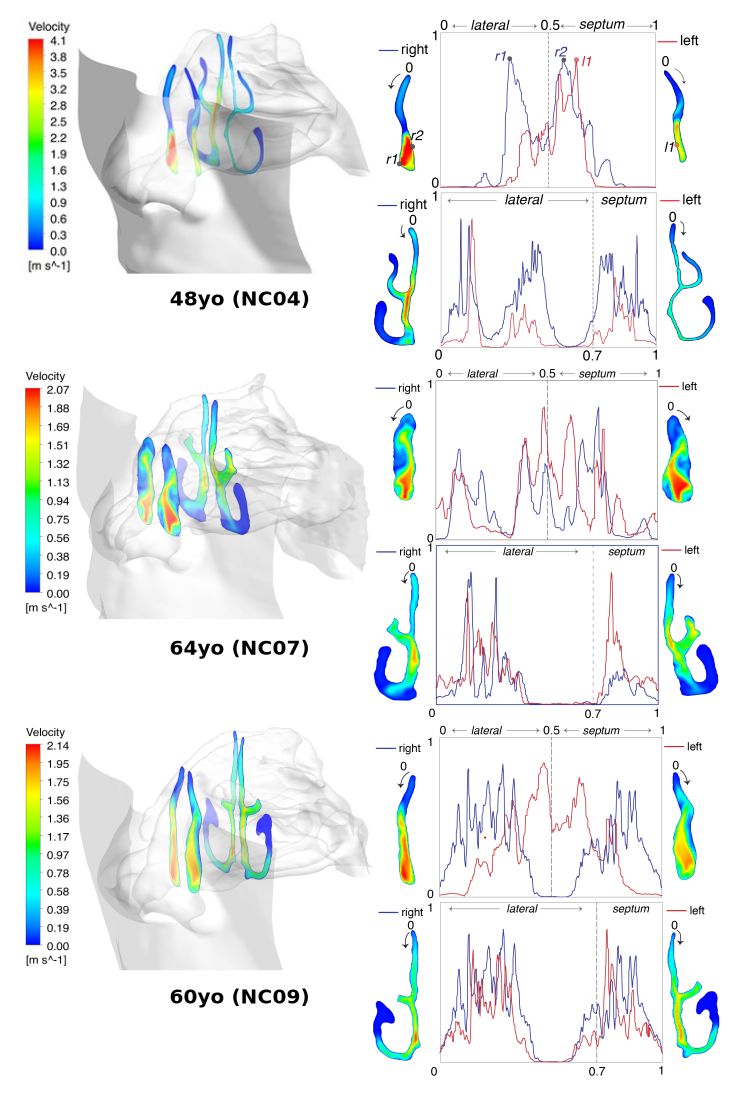
\includegraphics[width=\textwidth]{wsscs/wsscs1}
  \label{fig:wcs}
\end{figure}

\begin{figure} 
  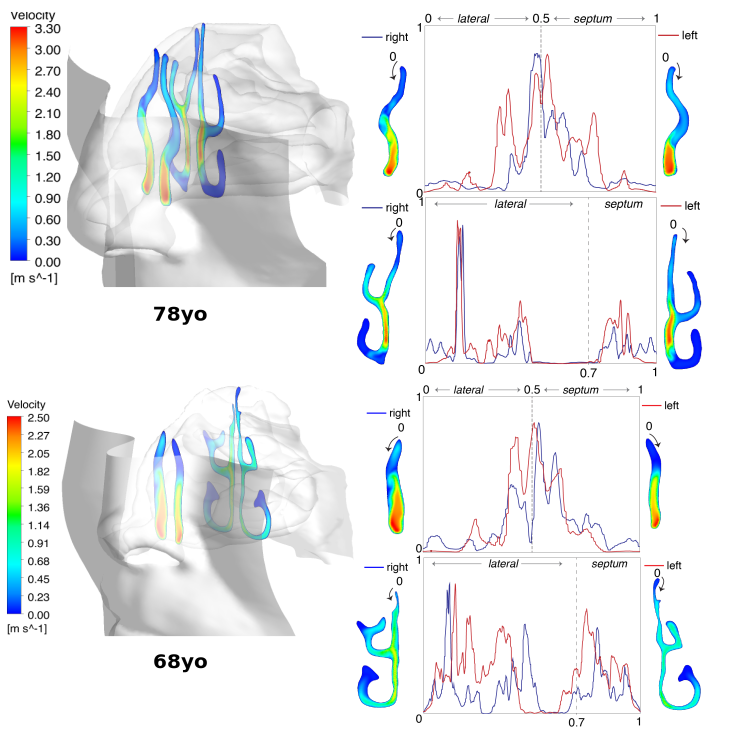
\includegraphics[width=\textwidth]{wsscs/wsscs2}
  \caption{Velocity contours and wall shear stress values along the perimeter outlines of two cross-sections. The x-axis is the perimeter distance starting from the top apex of each cross-section slice, and moves along the perimeter laterally. One full tracing around the perimeter is defined as 1.0. The dashed line represents the floor of the cross-section opposing its apex, and for the nasal valve, the halfway point \(0.5\), while for the turbinate cross-section it is 0.7. The y-axis represents normalized wall shear stress \(0 - 1\).}
  \label{fig:wcs}
\end{figure}

\begin{figure} 
  \includegraphics[width=\textwidth]{streamlines/sl1}
  \end{figure}

\begin{figure} 
  \includegraphics[width=\textwidth]{streamlines/sl2}
  \caption{Flow streamlines (coloured in blue) passing through the left and right chambers of the nasal cavity. Each chamber’s wall shear stress is shown (coloured in red).}
  \label{fig:vsl}
\end{figure}

In Figure \ref{fig:velcont} Streamlines are shown through the nasal chambers, coloured by velocity. In addition Sagittal contours of the vestibule, turbinal region and choannae are included.
\begin{figure} 
  \includegraphics[width=0.8\textwidth]{velcont}
  \caption{Streamlines through the cavities and sagittal contours taken at the nasal valve, turbinal region and choannae, coloured by normalised velocity magnitude.}
  \label{fig:velcont}
\end{figure}

\section{Heat and vapour transfer}

Some variation in the heat and vapour transfer efficacy can be seen between the models presented in this thesis. Note the higher than average figures for temperature and $H_2 O$ mass fraction in the valve area of the 78yo. In general the more voluminous models exhibit lower humidity and temperature (Figures \ref{fig:h2o} and \ref{fig:Temp}). The data from the atrophic rhinitis study by Garcia et al \cite{Garcia2007} is also included for comparison. Clearly the impact of the geometric variations associated with atrophic rhinitis on heat and vapour transfer are much more pronounced than that of the more voluminous older cavities when compared with the thinner cavities presented here. 

\begin{figure} 
  \includegraphics[width=\textwidth]{h2o}
  \caption{Average mass fraction of $\mathrm{H_2 O}$ as a function of normalised saggital position}
  \label{fig:h2o}
\end{figure}


\begin{figure} 
  \includegraphics[width=\textwidth]{Temperature}
  \caption{Average ambient temperature as a function of normalised saggital position}
  \label{fig:Temp}
\end{figure}


\chapter{Discussion}


The relationships between age and geometry have been investigated thoroughly through significant samples in previous studies using acoustic rhinometry \cite{Kalmovich2005, WhanKim2007, Edelstein1996}. What can be seen in the results from this study is the impact of the variation of geometry, in particular volume, on the air flow patterns within the cavity. 

What can be observed here in the geometries that cannot be observed through acoustic rhinometry is the surface area of the models. This allows the effective diameter to be calculated.  It can be seen that since the increase in the nasal volume is derived from a widening of the cavities, the surface area is effected significantly less than the volume, leading to increased effective diameter, which has been suggested to cause to increase vorticity in the cavities \cite{Garcia2007}.

The static pressure variation shown in figure \ref{fig:stpr} merits some discussion. Although it would seem logical that an increased cavity volume would have the effect of reducing pressure drop, this is not the result that has been recorded by previous researchers using rhinomanometry \cite{Lindemann2008}. This discrepancy is possibly due to the flexibility of the nasopharynx, varying the diameter of the exit in ways that are not replicated in the ct models.

The more even distribution of wall shear stress - both sagittally, as seen in Figures \ref{fig:wcont} and \ref{fig:wax}; and coronally, as seen in Figures \ref{fig:wcs} and \ref{fig:wcst} - is indicative of variations in airflow structure and therefore performance of the nasal cavity models. In particular the variation in the local maxima for WSS found in the region of the nasal valve is indicative of varying air conditioning capacity.

It seems in particular that it is only in the more severely enlarged cavities that drastically increased vorticity is seen in the air flow structures. The volume of the NC07 model of 55.07 $cm^3$, however is not a-typical of specimens of this age range, with a study of 81 men reporting an average volume for males between 65 and 79 of 56.7 $cm^3$\cite{Kalmovich2005}.

It seems probable that these marked increases in vorticity are linked to the observed reductions in air-conditioning functionality in specimens from this age group \cite{Lindemann2009a}. This is in accordance with the findings of \cite{Garcia2007} in relation to atrophic rhinitis patients. The model in their study had a recorded volume of 34.5 $cm^3$, however this was only measured to the end of the septum, and a comparison with the models from this study, as seen in figure ~\ref{fig:area} shows that the volume through the turbinal region of the atrophic rhinitis model was significantly larger than that of the largest model from this study, NC07. Although a quantity is not given for the volume of the nasopharynx in the atrophic rhinitis model, qualitative comparison between the  images of the model and those of the models from this study seem to show that the significant expansion of the nasopharynx which is present in all of the elderly models was not present in the model of the younger (26 yo) atrophic rhinitis sufferer. 

previous research has suggested that the presence of significant vortices such as those seen in the larger of the models presented in this study is related to the impairment of air conditioning functionality. The specifics of this mechanism , however, are yet to be investigated, and this is a piece of work which should be completed in future. In addition, the impact of the observed variations in airflow structure on the ability of the nasal cavity to filter particles from the air has not been investigated, and this is also an area which could be of some significance.

The heat and vapour transfer figures show what seems to be close to an inverse linear relationship between the voluminousness of the cavities and their heat and vapour transfer efficacy. This relationship agrees well with the data from Garcia et al \cite{Garcia2007} taken from their atrophic rhinitis patient. This suggests that the mechanisms causing this reduced efficacy in the atrophic rhinitis patient are the same as those in elderly patients; this may imply that, for more extreme cases, that the surgical procedures implemented for atrophic rhinitis patients could also be effective for the elderly. It has been suggested by \cite{Lindemann2008} that heat and vapour transfer are significantly effected by the minimal cross sectional area. The current data doesn't show anything to support or disprove this suggestion, as in general the models presenting higher mcas are also presenting higher voluminousness. In fact, the model that shows the highest MCA relative to its voluminousness [NC09], shows very good heat and vapour transfer.


\chapter{Conclusion}

Aberrations in nasal cavity form and functionality associated with the ageing process are important issues. 
Their importance is growing as the global population ages.
The underlying mechanisms behind many nasal cavity pathologies associated with the ageing process are still largely unknown.

This thesis presents findings from a set of preliminary investigations into in to older nasal cavity anatomy and airflow characteristics.
Although the sample size here is limited, it provides some preliminary insights in to questions raised by previous experimental results looking at the effects of old age on nasal cavity geometry and airflow.

In particular it provides a clear mechanistic alternative take on the relationship between geometry and nasal resistance to that provided by previous investigations using rhinomanometry and acoustic rhinometry. These (rhinomanometry and acoustic rhinometry) results show no clear relationship between cavity volume and resistance, whereas our computational investigation shows a clear relationship. Although a definitive answer is not offered as to the nature of the observed discrepency in findings, it does serve to identify the lack of understanding of this area in the current literature.

This thesis also provides a first look at mechanistic variations in older nasal cavity airflow, as well as previously unseen details regarding geometric formations. A circularity factor is introduced to quantify variations in shape between cavities for the anterior, middle and posterior nasal cavity regions.

Significant variations in flow concentration and developement are seen between the more and less voluminous cavities, particularly in regions such as the nasal valve, cited as being of particular significance to flow developement. The impact of this on flow developement is clearly seen in Figure \ref{fig:peakvel}, where a clear relationship is seen between valve cross sectional area and overall peak velocity.

Preliminary examinations are made into heat and vapour transfer within the cavities, suggestion some relationship between geometry and these functions in the nasal cavity.

\section{Future works}
The first gap left answered by this thesis is as to the validity of the results for the more voluminous cavities.
Although the results make sense when compared with previous results from rhinomanometry, as well as pipe flow theory, for completeness the results should be validated experimentally.

Another significant area which should be investigated is the impact of the aberrations observed in this thesis on particle deposition zones in the nasal cavity.
This area is significant for both olfaction and particle filtration.
It is the hope and intention of the author of this thesis that the preliminary insights presented here will lay the groundwork for future developments in the field of geriatric rhinology.


\bibliographystyle{unsrt}

\bibliography{chapters/database}

\end{document}
